\documentclass{article}
\usepackage{malmacros}
\begin{document}

\section{Model capacity and under/overfitting}

This section will dive deeper into the concept of under/overfitting, and explain the usage of these concepts. Using a linear model there will often be underfitting, but a polynomial model has a higher danger of overfitting. It has tendency to learn the noise of the data that it was trained with.


\subsection{Qa Explain the polynomial fitting via code review}

This section will explain the following code, and how it is implemented. The outcomes of the plots will also be described. 
\\ \\

The first interesting part is the following code:

\begin{pyminted}
def true_fun(X):
    return np.cos(1.5 * np.pi * X)

def GenerateData(n_samples = 30):
    X = np.sort(np.random.rand(n_samples))
    y = true_fun(X) + np.random.randn(n_samples) * 0.1
    return X, y
\end{pyminted}

The true function is  the actual function that the training data is trying to replicate, and the GenerateData function will use the true function as well as random values (noise) to simulate some data that will slightly resemble the true function. The X values are randomly generated, but sorted as well to have a proper simulated data set. 
\noindent
The following code dives deeper into the actual calculation of the scores:

\begin{pyminted}
np.random.seed(0)

X, y = GenerateData()
degrees = [1, 4, 15]

for i in range(len(degrees)):
    ax = plt.subplot(1, len(degrees), i + 1)
    plt.setp(ax, xticks=(), yticks=())

    polynomial_features = PolynomialFeatures(degree=degrees[i], include_bias=False)
    
    linear_regression = LinearRegression()
    pipeline = Pipeline([
            ("polynomial_features", polynomial_features),
            ("linear_regression", linear_regression)
        ])
    pipeline.fit(X[:, np.newaxis], y)

    # Evaluate the models using crossvalidation
    scores = cross_val_score(pipeline, X[:, np.newaxis], y, scoring="neg_mean_squared_error", cv=10)
    
    score_mean = -scores.mean()
    print(f"  degree={degrees[i]:4d}, score_mean={score_mean:4.2f},  {polynomial_features}")   

    X_test = np.linspace(0, 1, 100)
    y_pred = pipeline.predict(X_test[:, np.newaxis])
    
    # Plotting details
    ...
    ...
\end{pyminted}

The code will iterate through the length of degrees, which is 3. It will iterate through the degrees of 1, 4 and 15 respectively. It calculates the PolynomialFeatures for a degree. This means it will transform the training data, adding the 1st, 4th and 15th degrees polynomial of each feature in the training set as a new feature, respectively. This makes it possible to use LinearRegression with a pipeline. The pipeline will takes the polynomial features and the linear regression model. After it will be fitted, and the scores are calculated used cross val score. It has to be noted that the 'scoring' parameter is set to negate the mean squared error, meaning the higher the square error is, the better the model performs.
\\ \\
Hereafter a test data (from 0 to 1 with a 100 samples) is generated. The test data is used to calculate y pred, and the X test values and y pred are used to plot the following figures.

\begin{figure}[H]
  \centering
    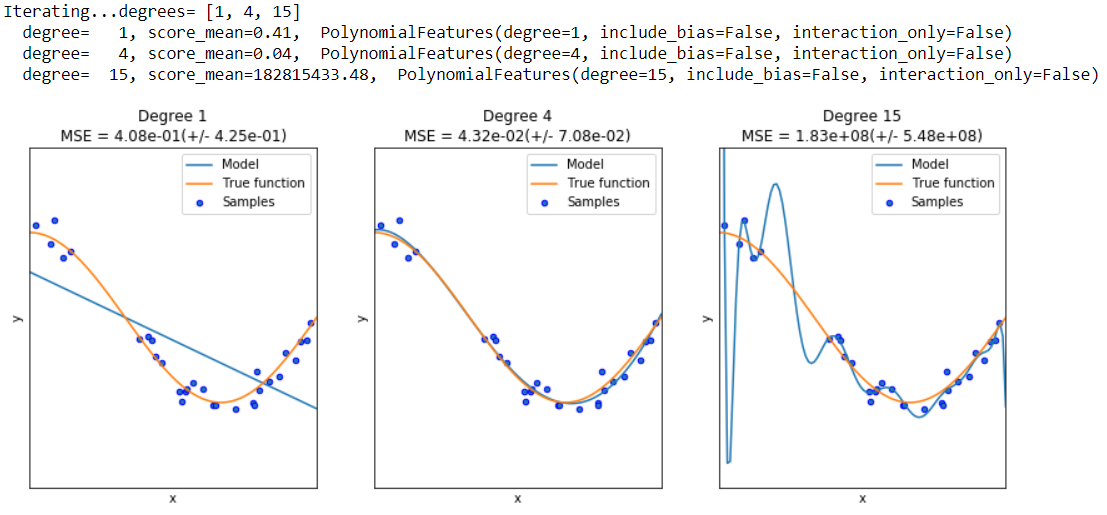
\includegraphics[width=1\textwidth]{sec5-cap-a}
    \caption{First model is underfitting, second one is  just right, third is overfitting}
    \label{fig:cap_a}
\end{figure}

Figure \ref{fig:cap_a} shows the output of the function iterating through the 3 degrees: 1, 4 and 15. The first degree is linear and will try to fit the data, but clearly not well enough. This is called underfitting. The score is also calculated as being 0,41, which is not extremely bad nor good. 
\\ \\
The 4th degree matches the true function quite well. It follows the path almost identically. The score is also calculated to be very low (almost perfect) to 0,04. It is not underfitting nor overfitting.
\\ \\
The last degree being 15 is trying to match every point in the training set. It has en extremely high score, meaning it is overfitting the training data extremely. This is happening because the 15th polynomial has too many free degrees to play with. The first degree had too little and the 4th degree had  just enough to fit the training data pretty much perfectly. 

\subsection{Qb Explain the capacity and under/overfitting concept}

The first plot of figure  \ref{fig:cap_a} shows that the model has been fit with the training data, but it is impossible for the degree of 1 to ever fit to the true function properly, because it can only fit the data in a straight line. The \textit{capacity} of this model is hence 1. The capacity tells how well the model can fit the data. Since the model is a bit more complex than a degree of 1, this model will perform poorly and \textit{underfit} the data. This  means a capacity of 1 is not good enough for the model.
\\ \\
The next plot, however, is using a degree of 4. This means the capacity is 4, and much higher than a capacity of 1. The model has a much higher chance of actually fitting the training test properly, since it has a higher degree of movement. This is a perfect capacity for this model.
\\ \\
The last plot has a degree of 15 - a capacity of 15. This means it can fit many more elements than the previous elements. However, this will mean that it can (and will) try to fit every since data point in the set. This is a problem, because since it will fit every point, it can also go after potential outliers, and thus \textit{overfit} the data. The model have a high capacity and can thus overfit the data by learning characteristics that are not usual for the whole data set. It does not have a clear picture of the entire data set, but simply the points themselves.
\\ \\
This means that the potential for overfitting will occur with higher capacities, and underfitting can occur when using lower capacities. 


\end{document}